\documentclass[a4paper, 12pt]{article} % Tipo do arquivo
\usepackage[utf8]{inputenc} % Fonte
\usepackage[T1]{fontenc} % Fonte
\usepackage[top=3.0cm,bottom=2.0cm,left=2.0cm,right=2.0cm, headheight=1.5cm]{geometry} % Formatação e margem
\usepackage{fancyhdr} % Cabeçalhos e rodapés
\usepackage[brazilian]{babel} % Deixa em português
\usepackage{enumitem} % Enumeração
\usepackage{siunitx}
\usepackage{graphicx} % Imagens
\usepackage{amsmath, amsfonts, amsthm, amssymb, bigints, physics} % Coisas da matemática
\usepackage{indentfirst} % Identar primeiro parágrafo 
\usepackage{float} % Formatação de Tabelas e Figuras
\usepackage{lipsum} % Dummy text generator
\usepackage{url}
\usepackage{amsmath}
\usepackage{titlesec}
\usepackage{makecell}
\titlelabel{\thetitle.\enskip}
\pagestyle{fancy}
\usepackage{booktabs}
\renewcommand{\footrulewidth}{.3pt}
\renewcommand{\headrulewidth}{.3pt}
\usepackage{caption} 
\usepackage{float}
\usepackage{arydshln}
\usepackage{booktabs}
\usepackage{multirow}

\pagestyle{fancy} 
\renewcommand{\footrulewidth}{.3pt} 
\renewcommand{\headrulewidth}{.3pt} 
\lhead{
\includegraphics[height=1.2cm]{images/ITA.png}\vspace*{0.1cm}} 
\chead{\large CMC-12 - Exame Final \vspace*{0.1cm}} 
\rhead{} 
\cfoot{\thepage}

% Início do documento 
\begin{document} 
\thispagestyle{empty} 
\vspace*{2.15cm}

% Logo ITA
\begin{figure}[htb]
    \centering
    
\includegraphics[scale=0.52]{images/ITA.png}
    
    \large Instituto Tecnológico de Aeronáutica
\end{figure}

\begin{center}
    \huge{CMC-12 – Exame Final} 
    
    \vspace{.5cm}
    \large Prof. Marcos Ricardo Omena de Albuquerque Maximo
    
    \vspace{1cm}
    \Huge Controlador Não Linear de Barra Articulada
    
    \vspace{.5cm}
    \Large Julho de 2025
    
    \vspace{.15cm}
    \large
    Danilo Miranda Oliveira \\
    Geison Vasconcelos Lira Filho \\
    José Alberto Feijão Tizon \\
\end{center}

\newpage
\setcounter{page}{1}


\section{Introdução}

Este relatório apresenta o projeto final desenvolvido na disciplina CMC-12, cujo objetivo é implementar e analisar um controlador não linear para o sistema que consiste em uma barra articulada sobre a qual uma argola pode deslizar livremente, sem atrito. O controle atua sobre o torque aplicado à barra, visando posicionar a argola em uma posição desejada \( x_r \) ao longo da barra, utilizando como única força externa a gravidade.

A solução implementada para projetar o controlador desse sistema permite que o projetista determine o tipo de controlador -- entre P, PI, PD, DI e PID -- e escolha três tipos de combinação de requisitos no domínio do tempo, sobressinal + tempo de subida, sobressinal + tempo de acomodação e sobressinal + tempo de pico, para posicionar a argola numa barra infinita. Desse modo, é possível determinar o controlador mais eficaz para a barra do tamanho que se deseja projetar e verificar se os requisitos podem ser obedecidos para todas as posições da barra que se deseja projetar.



\section{Descrição do Sistema}

\subsection{Modelagem Física}

O sistema físico analisado consiste em uma barra rígida, com momento de inércia \( J \), articulada na posição \( x = 0 \) e assumida como infinitamente longa. Solidária a essa barra, uma argola de massa \( m \) desliza livremente, sem atrito. O controle do sistema é realizado por meio da aplicação de um torque \( \tau(t) \) na base da barra, o qual altera seu ângulo \( \theta(t) \) em relação à vertical. A única força externa considerada na modelagem é a força gravitacional atuando sobre a argola.

\subsection{Equações Dinâmicas Não Lineares}

No referencial solidário à barra, as forças atuantes sobre a argola ao longo do eixo \( x \) são a componente da força gravitacional, expressa como \( -mg \sin(\theta) \), e a força centrífuga decorrente da rotação da barra, dada por \( m \dot{\theta}^2 x \). Como se desprezam os atritos e forças perpendiculares à barra, como as forças de Coriolis e de Euler, que não influenciam a movimentação ao longo do eixo \( x \), a equação de movimento da argola no referencial rotativo é representada por:

\begin{equation}
    m \ddot{x} = -mg \sin(\theta) + m \dot{\theta}^2 x
\end{equation}

A dinâmica de rotação da barra é modelada por:

\begin{equation}
    \tau(t) = J \ddot{\theta}
\end{equation}

\subsection{Linearização via Espaço de Estados}

Para fins de análise e projeto de controladores lineares, é conveniente representar a dinâmica do sistema em espaço de estados. A partir do modelo não linear previamente obtido, consideram-se as seguintes equações que descrevem a dinâmica da argola e da barra:

\begin{align}
    m \ddot{x} &= -mg \sin(\theta) + m \dot{\theta}^2 x \label{eq:ddotx_nl} \\
    J \ddot{\theta} &= \tau \label{eq:ddottheta}
\end{align}

Definimos o vetor de estados como \( \mathbf{x} = [x \quad \dot{x} \quad \theta \quad \dot{\theta}]^\top \), a entrada como \( u = \tau \), e consideramos como saída a posição da argola \( y = x \).

A equação \eqref{eq:ddotx_nl}, dividida por \( m \), fornece:

\begin{equation}
    \ddot{x} = -g \sin(\theta) + \dot{\theta}^2 x
\end{equation}

De forma semelhante, da equação \eqref{eq:ddottheta}, temos:

\begin{equation}
    \ddot{\theta} = \frac{1}{J} \tau
\end{equation}

Substituindo as variáveis de estado, o sistema dinâmico pode ser reescrito como:

\begin{align}
    \dot{x}_1 &= x_2 \\
    \dot{x}_2 &= -g \sin(x_3) + x_4^2 x_1 \\
    \dot{x}_3 &= x_4 \\
    \dot{x}_4 &= \frac{1}{J} u
\end{align}

Com isso, obtém-se o modelo de espaço de estados não linear na forma compacta:

\begin{equation}
    \dot{\mathbf{x}} = f(\mathbf{x}, u), \quad y = h(\mathbf{x})
\end{equation}

Para linearizar o sistema, realiza-se uma expansão em série de Taylor de primeira ordem das funções \( f(\mathbf{x}, u) \) e \( h(\mathbf{x}) \) em torno do ponto de equilíbrio \( \mathbf{x}_e = \mathbf{0} \), \( u_e = 0 \). As matrizes do modelo linearizado são dadas por:

\begin{align}
    A &= \left.\frac{\partial f}{\partial \mathbf{x}}\right|_{\mathbf{x}_e, u_e} \qquad 
    B = \left.\frac{\partial f}{\partial u}\right|_{\mathbf{x}_e, u_e} \\
    C &= \left.\frac{\partial h}{\partial \mathbf{x}}\right|_{\mathbf{x}_e} \qquad\quad
    D = \left.\frac{\partial h}{\partial u}\right|_{u_e}
\end{align}

Calculando essas derivadas parciais, obtêm-se as seguintes matrizes:

\[
A = \begin{bmatrix}
0 & 1 & 0 & 0 \\
0 & 0 & -g & 0 \\
0 & 0 & 0 & 1 \\
0 & 0 & 0 & 0
\end{bmatrix}, \quad
B = \begin{bmatrix}
0 \\
0 \\
0 \\
\frac{1}{J}
\end{bmatrix}, \quad
C = \begin{bmatrix}
1 & 0 & 0 & 0
\end{bmatrix}, \quad
D = [0]
\]

Esse modelo linearizado descreve a dinâmica do sistema nas proximidades do ponto de equilíbrio. Ele será utilizado para o projeto dos controladores lineares na malha externa, uma vez que fornece uma aproximação acurada do comportamento local do sistema não linear original. A partir da modelagem em espaço de estados e da posterior aplicação de uma expansão em série de Taylor de primeira ordem em torno do ponto de equilíbrio \((\theta, \dot{\theta}, x, \dot{x}) = (0, 0, 0, 0)\), obtêm-se as equações linearizadas que descrevem a dinâmica local do sistema. Considerando pequenas oscilações e desprezando termos não lineares de ordem superior, a dinâmica reduz-se às seguintes equações diferenciais lineares:

\begin{equation}
    \ddot{x} = -g \cdot \theta
\end{equation}
\begin{equation}
    \ddot{\theta} = \frac{1}{J} \cdot \tau
\end{equation}

Essas expressões representam, respectivamente, a aceleração da argola em função da inclinação da barra e a aceleração angular da barra em função do torque aplicado. Tal forma linearizada é essencial para a síntese de controladores clássicos baseados em modelos lineares, como controladores PID ou estratégias de realimentação de estados.



\section{Projeto do Controlador}

\subsection{Estrutura em Malha Interna e Externa}
Devido à natureza hierárquica do sistema, em que a posição \( x \) depende do ângulo \( \theta \), que por sua vez depende do torque \( \tau \), adota-se uma abordagem com duas malhas de controle. A malha interna, mais rápida, é responsável por controlar o ângulo da barra a partir do torque aplicado. Para isso, utiliza-se um controlador proporcional com compensação de velocidade (P+V). Já a malha externa, mais lenta, controla a posição da argola ao longo da barra. São testados diferentes controladores (P, PI, PD, DI e PID), todos com pré-filtro na referência para eliminação dos zeros, de forma que seja possível estabelecer uma dinâmica de segunda ordem padrão aproximada para esses controladores.

\subsection{Controladores Utilizados nas Malhas}

A arquitetura de controle adotada é composta por uma estrutura hierárquica com duas malhas principais. A malha externa é responsável pelo controle da posição da argola e utiliza um controlador PID clássico, atuando sobre o erro de posição para gerar uma referência angular. Já a malha interna é dedicada ao controle da orientação da barra e implementa uma estratégia do tipo P+V. Essa estratégia consiste em duas realimentações aninhadas: uma proporcional sobre o ângulo da barra e outra proporcional sobre sua velocidade angular, funcionando respectivamente como ações de posição e velocidade.

Para o cálculo dos ganhos dos controladores, considera-se o modelo linearizado do sistema, no qual as não linearidades e forças centrífugas são desprezadas. Os parâmetros são calculados de forma analítica, a partir dos requisitos de desempenho definidos para o sistema. Posteriormente, o projeto é validado no ambiente Simulink, onde o modelo exato do sistema é simulado, incluindo as não linearidades e a força centrífuga que foram omitidas na linearização. Dessa forma, verifica-se se o controlador projetado atende adequadamente ao desempenho esperado quando aplicado ao sistema real.

\subsection{Compensador PID e pré-filtro}

No ambiente do simulink, foram configurados dois blocos referentes à malha externa de posição, um dos blocos consiste em um pré-filtro para a eliminação dos zeros das funções de transferência e outro referentes ao controlador PID geral. A função de transferência da posição $x$ em relação ao referencial $x_r$ é mostrada na equação abaixo.

\[(x_r\cdot F(s)-x)\cdot C(s)\cdot\frac{g}{s^2}=x\]

Em que $x_r$ é a referência de posição, $g$ é gravidade, $C(s)$ é o compensador PID e $F(s)$ é o pré-filtro. As estruturas do pré-filtro e do compensador respectivamente, são apresentas nas equações abaixo. Se deseja-se um controlador PID, calcula-se

\[F(s) = \frac{fK_ps+K_i}{K_ds^2+K_ps+K_i}\]
\[C(s)=\frac{K_ds^2+K_ps+K_i}{s}\]

Em que $K_d$, $K_p$ e $K_i$ são os ganhos do controlador PID e $f$ é um fator de correção do pré-filtro para que ele sempre elimine os zeros independente do tipo de controlador utilizado.

\subsection{Obtenção analítica de ganhos e definição do controlador}

Os ganhos foram projetados considerando-se sempre uma dinâmica de segunda ordem padrão baseado na combinação de requisitos e no tipo de compensador escolhidos. O valor de $M_p$ é o mesmo para as três combinações.
\[\xi = \frac{-ln(M_p)}{\sqrt{\pi^2+ln^2(M_p)}}\]
Caso escolha-se o tempo de subida, $\omega_n$ é dado pela equação abaixo.
\[\omega_n=\frac{\pi-arccos(\xi)}{t_r\sqrt{1-\xi^2}}\]
Caso escolha-se o tempo de pico, temos a equação abaixo.
\[\omega_n=\frac{\pi}{t_p\sqrt{1-\xi^2}}\]
Por fim, caso seja feita a escolha do tempo de acomodação, obtemos omega pela expressão abaixo.
\[\omega_n=\frac{3}{\xi t_s}\]
Com os termos da equação de segunda ordem padrão definidos, é possível determinar os ganhos com base neles. Para um compensador P, fazemos $K_i=0$ e $K_d=0$ e escolhemos o fator $f=1$, assim o pré filtro, o compensador e a equação final do controlador em malha fechada são dados respectivamente pelas equações abaixo.

\[F(s)=1\]
\[C(s)=K_p\]
\[G(s)=\frac{K_p}{\frac{1}{g}s^2+K_p}\]

Assim, considerando uma dinâmica de segunda ordem, obtemos que o ganho $K_p$ é dado pela equação abaixo.
\[K_p=\frac{\omega_n^2}{g}\]
Esse sistema é marginalmente estável, devido a seus polos no eixo imaginário, ele não diverge para infinito mas oscila infinitamente, não atingindo estabilidade e não sendo adequado para uso como controlador, mas ainda assim ele foi incluído no projeto para evidenciar sua inadequação e sua diferença em relação a outros controladores. Para um compensador PD, fazemos $K_i=0$ e escolhemos o fator $f=1$, assim o pré filtro, o compensador e a equação final do controlador em malha fechada são dados respectivamente pelas equações abaixo.

\[F(s)=\frac{K_p}{K_ds+K_p}\]
\[C(s)=K_ds+K_p\]
\[G(s)=\frac{K_p}{\frac{1}{g}s^2+K_ds+K_p}\]
Assim, considerando uma dinâmica de segunda ordem, obtemos que os ganhos $K_p$ e $K_d$ são dados pela equação abaixo.
\[K_d=\frac{2\xi\omega_n}{g}\]
\[K_p=\frac{\omega_n^2}{g}\]
Esse sistema, por apresentar zeros somente no semiplano esquerdo, é estável e atinge o equilíbrio em regime na referencia. Para um compensador PI, fazemos $K_d=0$ e escolhemos o fator $f=0$, assim o pré filtro, o compensador e a equação final do controlador em malha fechada são dados respectivamente pelas equações abaixo.

\[F(s)=\frac{K_i}{K_ps+K_i}\]
\[C(s)=\frac{K_ps+K_i}{s}\]
\[G(s)=\frac{K_i}{\frac{1}{g}s^3+K_ps+Ki}\]

Esse sistema tem três polos, porém o polo real não é distante o suficiente da origem para que os polos complexos sejam dominantes, de forma que esse sistema está sujeito a instabilidades de terceira ordem impossíveis de serem resolvidas. Além disso, os polos complexos conjugados estão no semiplano real positivo, de forma que o sistema é instável e não é adequado para ser usado como controlador, mas ainda assim ele foi incluído no projeto para evidenciar sua inadequação e sua diferença em relação a outros controladores. Mesmo assim, considerando uma dinâmica de segunda ordem, obtemos que os ganhos $K_p$ e $K_i$ são dados pelas equaçõess abaixo.
\[K_p=\frac{\omega_n^2-4\xi^2\omega_n^2}{g}\]
\[K_i=\frac{2\xi\omega_n^3}{g}\]

Para o compensador DI, fazemos $K_p=0$ e escolhemos o fator $f=0$, assim o pré filtro, o compensador e a equação final do controlador em malha fechada são dados respectivamente pelas equações abaixo.
\[F(s)=\frac{K_i}{K_ds^2+K_i}\]
\[C(s)=\frac{K_ds^2+K_i}{s}\]
\[G(s)=\frac{K_i}{\frac{1}{g}s^3+K_ds^2+K_i}\]
Esse sistema apresenta a mesma estrutura de polos do compensador PI, o polo real é próximo da origem de forma que os polos complexos não são dominantes, e os polos complexos estão no semiplano real positivo, de forma que esse controlador é instável e não é adequado para uso, mas ainda assim ele foi incluído no projeto para evidenciar sua inadequação e sua diferença em relação a outros controladores. De qualquer modo, os ganhos $K_d$ e $K_i$ são dados pelas equações abaixo.
\[K_d=\frac{\omega_n-4\xi^2\omega_n}{2\xi g}\]
\[K_i=\frac{\omega_n^3}{2\xi g}\]
Por fim, para o compensador PID, escolhemos o fator $f=0$, assim o pré filtro, o compensador e a equação final do controlador em malha fechada são dados respectivamente pelas equações abaixo.
\[F(s)=\frac{K_i}{K_ds^2+K_ps+K_i}\]
\[C(s)=\frac{K_ds^2+K_ps+K_i}{s}\]
\[G(s)=\frac{K_i}{\frac{1}{g}s^3+K_ds^2+K_ps+K_i}\]
Com três ganhos, o polo real não fica determinado com base nos outros polos, de forma que podemos escolhê-lo de forma que os polos complexos sejam dominantes, além disso, os polos complexos estão no semiplano real negativo, o que indica que esse sistema é adequado para ser utilizado como controlador. Os ganhos $K_d$, $K_p$ e $K_i$ respectivamente são dados pelas equações abaixo.
\[K_d=\frac{7\xi\omega_n}{g}\]
\[K_p=\frac{10\xi^2\omega_n^2+\omega_n^2}{g}\]
\[K_i=\frac{5\xi\omega_n^3}{g}\]
As equações dos ganhos com base nos requisitos foram implementadas no matlab para serem usadas no modelo geral do controlador.

\section{Resultados e Discussão}

\subsection{Comparação entre simuladores}

Inicialmente, foi realizada uma comparação entre os tipos de controladores disponíveis para analisar qual deles é capaz de estabilizar. Nesse teste, foi realizada a simulação do sistema para referência fixa $x_r = 0,9$ e com requisitos fixos, de modo que a resposta dos diferentes tipos de compensador podem ser observadas na figura \ref{fig:resultado-controladores}.

\begin{figure}[H]
    \centering
    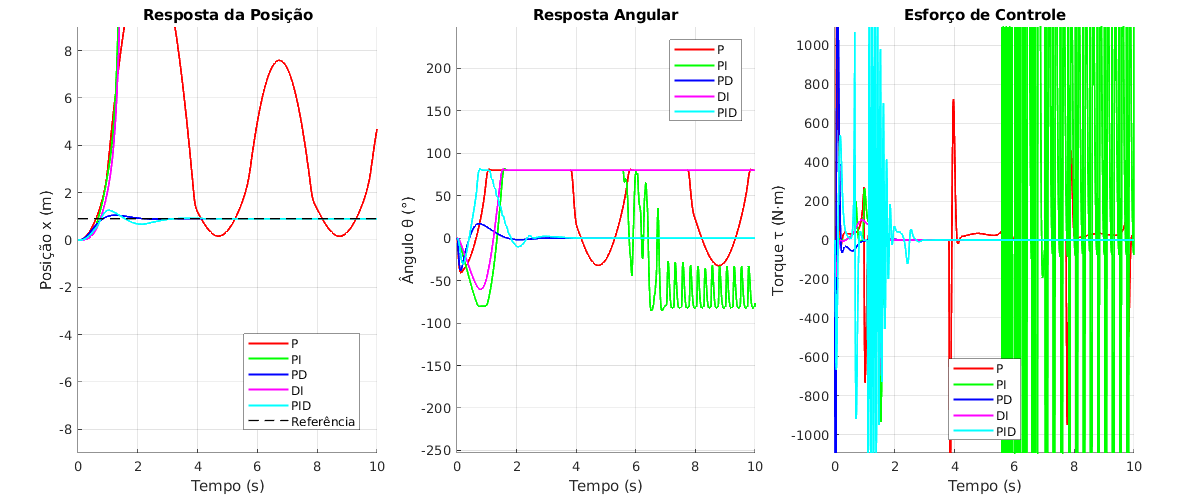
\includegraphics[width=0.8\textwidth]{images/comparar-controlador.png}
    \caption{\centering Análise do comportamento do sistema para os diferentes tipos de controladores}
    \label{fig:resultado-controladores}
\end{figure}

Observa-se, na resposta de posição, que os controladores PD e PID são os únicos capazes de rastrear corretamente a referência, promovendo estabilização e erro de regime próximo de zero. Entre eles, o controlador PD apresentou o *melhor desempenho global*, com rápida convergência, menor sobrelevação e uso mais eficiente do esforço de controle.

O controlador P resultou em um sistema *marginalmente estável*, caracterizado por oscilações sustentadas e ausência de amortecimento. Apesar de não divergir, o sistema não converge para a referência, evidenciando a limitação dessa estrutura em sistemas com dinâmicas acopladas.

Os controladores PI e DI mostraram-se totalmente instáveis, apresentando crescimento exponencial da posição e do ângulo, com comportamento divergente e torques irrealisticamente elevados. Tal comportamento inviabiliza sua aplicação em qualquer cenário realista.

Na resposta angular, o PD se destaca novamente, controlando o ângulo da barra de forma suave e eficiente. O PID, embora estável, apresentou resposta mais lenta e esforço de controle mais elevado que o PD, além de apresentar mais oscilação para estabilizar na posição de referência.

\subsection{Avaliação de diferentes referências}

\begin{figure}[H]
    \centering
    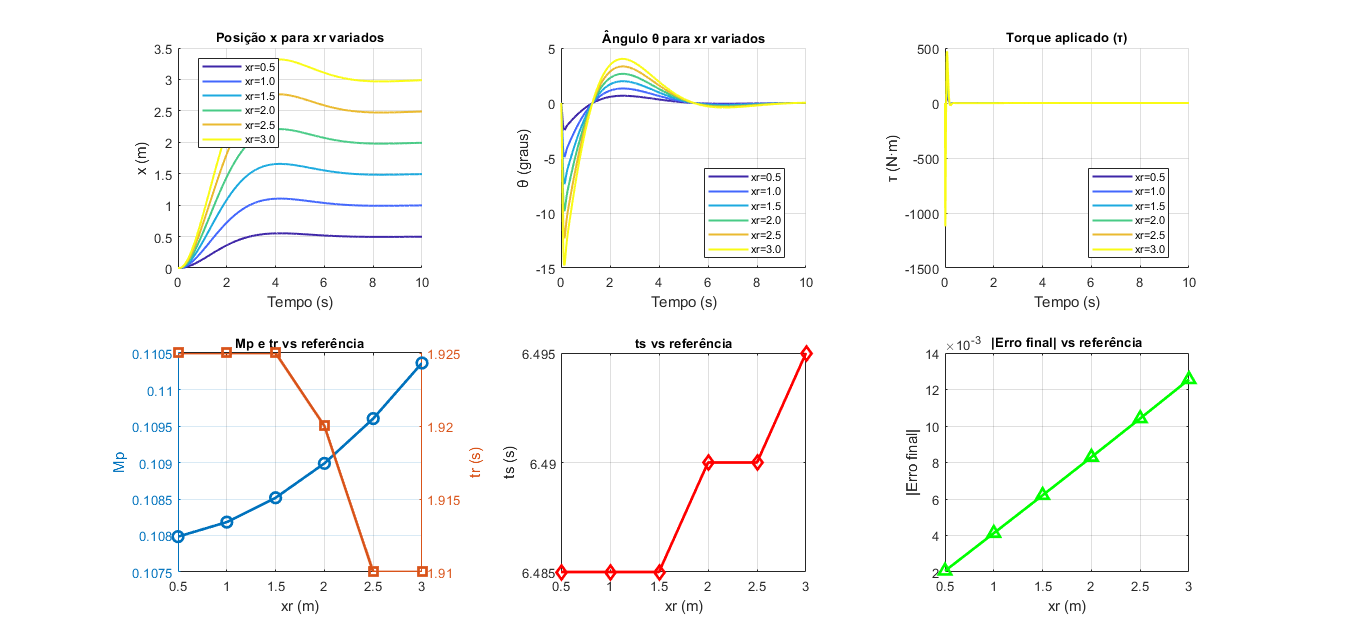
\includegraphics[width=1.0\textwidth]{images/teste_xr_PD_tr_3.0_Mp_0.1.png}
    \caption{\centering Respostas ao degrau para diferentes valores de referência para o controlador PD com requisitos $M_p=0.1$ e $t_r=0.3s$}
    \label{fig:resultado-controladores}
\end{figure}

A figura acima mostra as respostas do controlador PD para diferentes valores de referência de posição ($x_r$). Observa-se que, à medida que $x_r$ aumenta, o sobressinal tanto da posição ($x$) quanto do ângulo ($\theta$) também cresce, o que indica que o sistema passa a oscilar mais antes de atingir o regime permanente. Esse comportamento pode ser problemático em algumas aplicações. A análise do torque aplicado reforça que a malha de controle do ângulo reage de forma significativamente mais rápida do que a da posição — o que é esperado, já que o projeto foi pensado com uma malha interna (para o ângulo) mais ágil, enquanto a malha externa (para a posição) atua de forma mais suave sobre a argola. No entanto, para valores maiores de $x_r$, o sistema tende à instabilidade, pois as oscilações se acentuam. Isso ocorre porque termos não lineares, como a força centrífuga, tornam-se mais relevantes em posições distantes do centro, afetando a eficácia do controlador linear. Assim, é fundamental validar o controlador em simulações que incluam o modelo não linear completo.

\subsection{Avaliação de diferentes tipos de requisitos}

% Sexta

\section{Conclusão}
O desenvolvimento deste projeto permitiu compreender os principais desafios envolvidos no controle de sistemas não lineares, especialmente na presença de malhas hierárquicas e interdependentes. A estratégia de controle adotada, com malhas interna e externa, mostrou-se efetiva para garantir o rastreamento da posição desejada pela argola, mesmo em condições adversas. Como possíveis extensões do trabalho, sugere-se a análise do sistema com perturbações externas, como atrito ou impa


\end{document}
